\begin{frame}[fragile]{Visualizing The Geometry}

  \begin{scriptsize}
    \begin{lstlisting}[language=XML,gobble=4]
      <?xml version="1.0"?>
      <plots>

        <plot id="1" type="slice" basis="xy" color="mat">
          <filename>plot_name</filename>
          <origin>0 0 0</origin>
          <width>155 155</width>
          <pixels>1000 1000</pixels>
        </plot>
        
      </plots>
    \end{lstlisting}
  \end{scriptsize}

  \begin{itemize}
    \item Any number of plots can be specified in \verb|plots.xml| 
    \item Plots are slices along the \verb|xy|, \verb|xz|, or \verb|yz| planes
    \begin{itemize}
      \item The user specifies the extents of the plotting window
      \item The user specified the pixel resolution of the plot
    \end{itemize}
    \item OpenMC generates a \verb|ppm| image - can be converted into \verb|png| to reduce size
  \end{itemize}
  
\end{frame}

%-------------------------------------------------------------------------------

\begin{frame}[fragile]{Plotting Options}

  \begin{scriptsize}
    \begin{lstlisting}[language=XML,gobble=4]
      <?xml version="1.0"?>
      <plots>

        <plot id="1" type="slice" basis="xy" color="mat">
          <filename>material_coloring</filename>
          <origin>0 0 0</origin>
          <width>155 155</width>
          <pixels>1000 1000</pixels>
        </plot>
        
        <plot id="2" type="slice" basis="xy" color="cell">
          <filename>cell_coloring</filename>
          <origin>0 0 0</origin>
          <width>155 155</width>
          <pixels>1000 1000</pixels>
        </plot>
        
      </plots>
    \end{lstlisting}
  \end{scriptsize}

  \begin{itemize}
    \item Can color by cell ID
    \begin{itemize}
      \item Repeated cells in lattices and fill cells have the same color
    \end{itemize}
    \item Can color by material ID
  \end{itemize}
  
  \onslide<2>{
    \setlength{\TPHorizModule}{\framewidth}
    \setlength{\TPVertModule}{\paperheight}
    \begin{textblock}{1}(0.12,-0.72)
      \begin{columns}[c]
      \column{2in}
      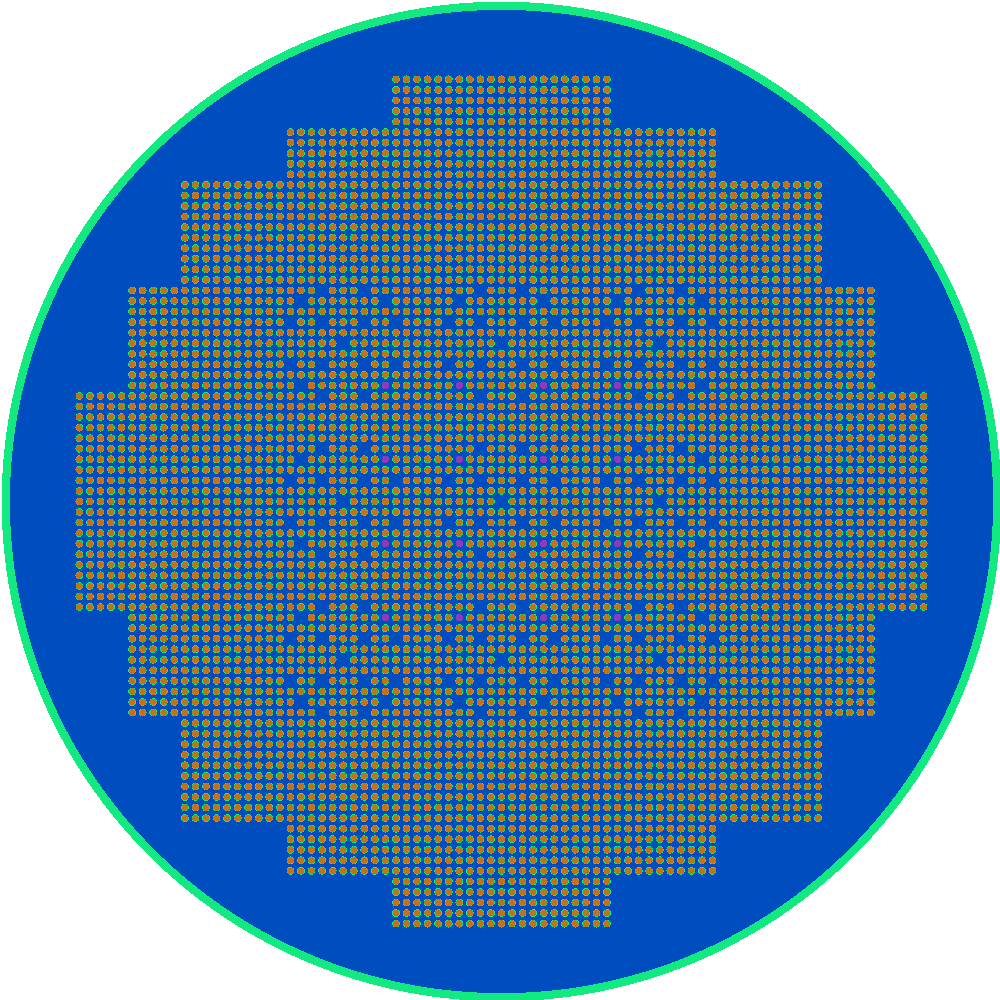
\includegraphics[width=2in]{src/plots/1_material_coloring.png}
      \column{3.5in}
      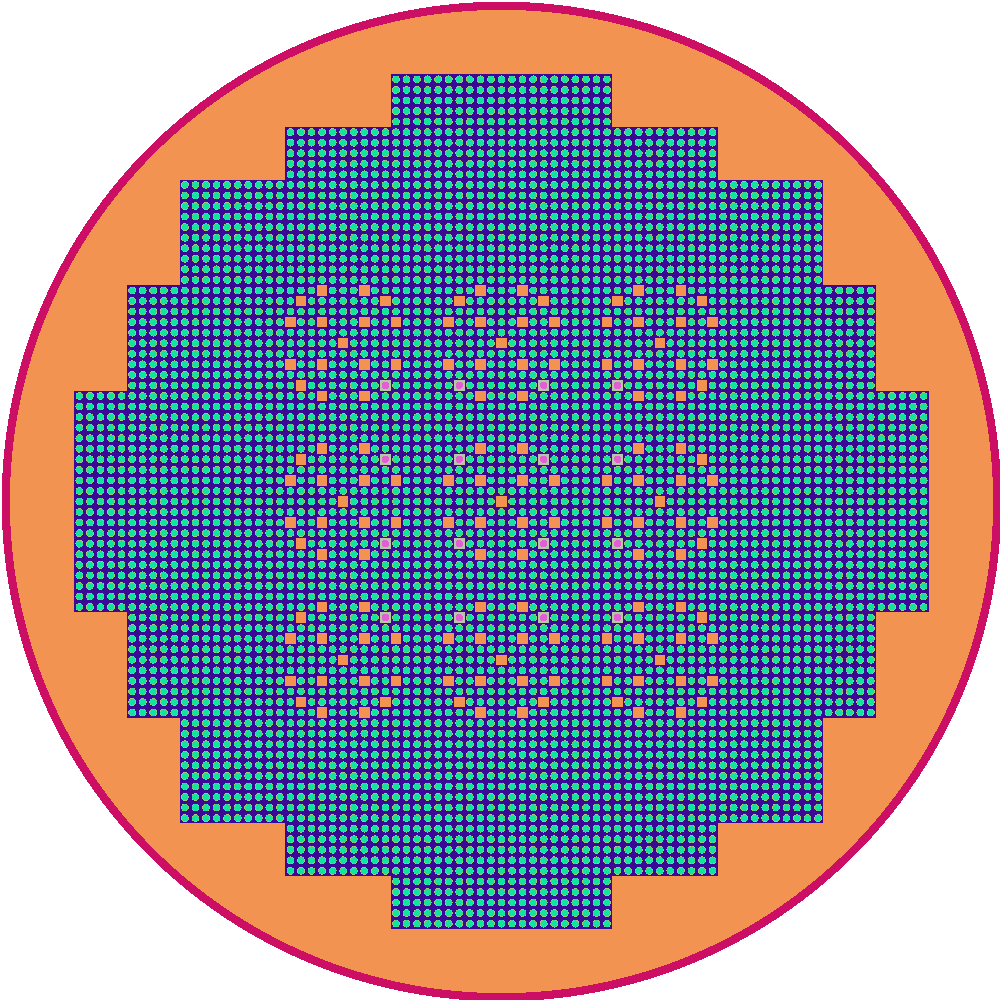
\includegraphics[width=2in]{src/plots/2_cell_coloring.png}
      \end{columns}
    \end{textblock}
  }
  
\end{frame}

%-------------------------------------------------------------------------------

\begin{frame}[fragile]{Plotting Options}

  \begin{scriptsize}
    \begin{lstlisting}[language=XML,gobble=4]
      <?xml version="1.0"?>
      <plots>

      <plot id="4" type="slice" color="mat">
        <filename>col_spec</filename>
        <origin>0 0 0</origin>
        <width>155 155</width>
        <basis>xy</basis>
        <pixels>2000 2000</pixels>
        <!-- Change background color to black -->
        <!-- This is the color used where no cell is found -->
        <background>0 0 0</background>
        <!-- Specify material colors -->
        <col_spec id="1" rgb="0 0 255"/>      <!-- Water: blue -->
        <col_spec id="2" rgb="255 0 0"/>      <!-- Fuel:  red  -->
        <col_spec id="3" rgb="160 160 160"/>  <!-- Clad:  gray -->
        <!--The remaining material colors will be randomly selected -->
      </plot>

      </plots>
    \end{lstlisting}
  \end{scriptsize}

  \begin{itemize}
    \item Can specify colors for cells or materials manually
  \end{itemize}
  
  \onslide<2>{
    \setlength{\TPHorizModule}{\framewidth}
    \setlength{\TPVertModule}{\paperheight}
    \begin{textblock}{1}(0.12,-0.645)
      \begin{columns}[c]
      \column{2in}
      \column{3.5in}
      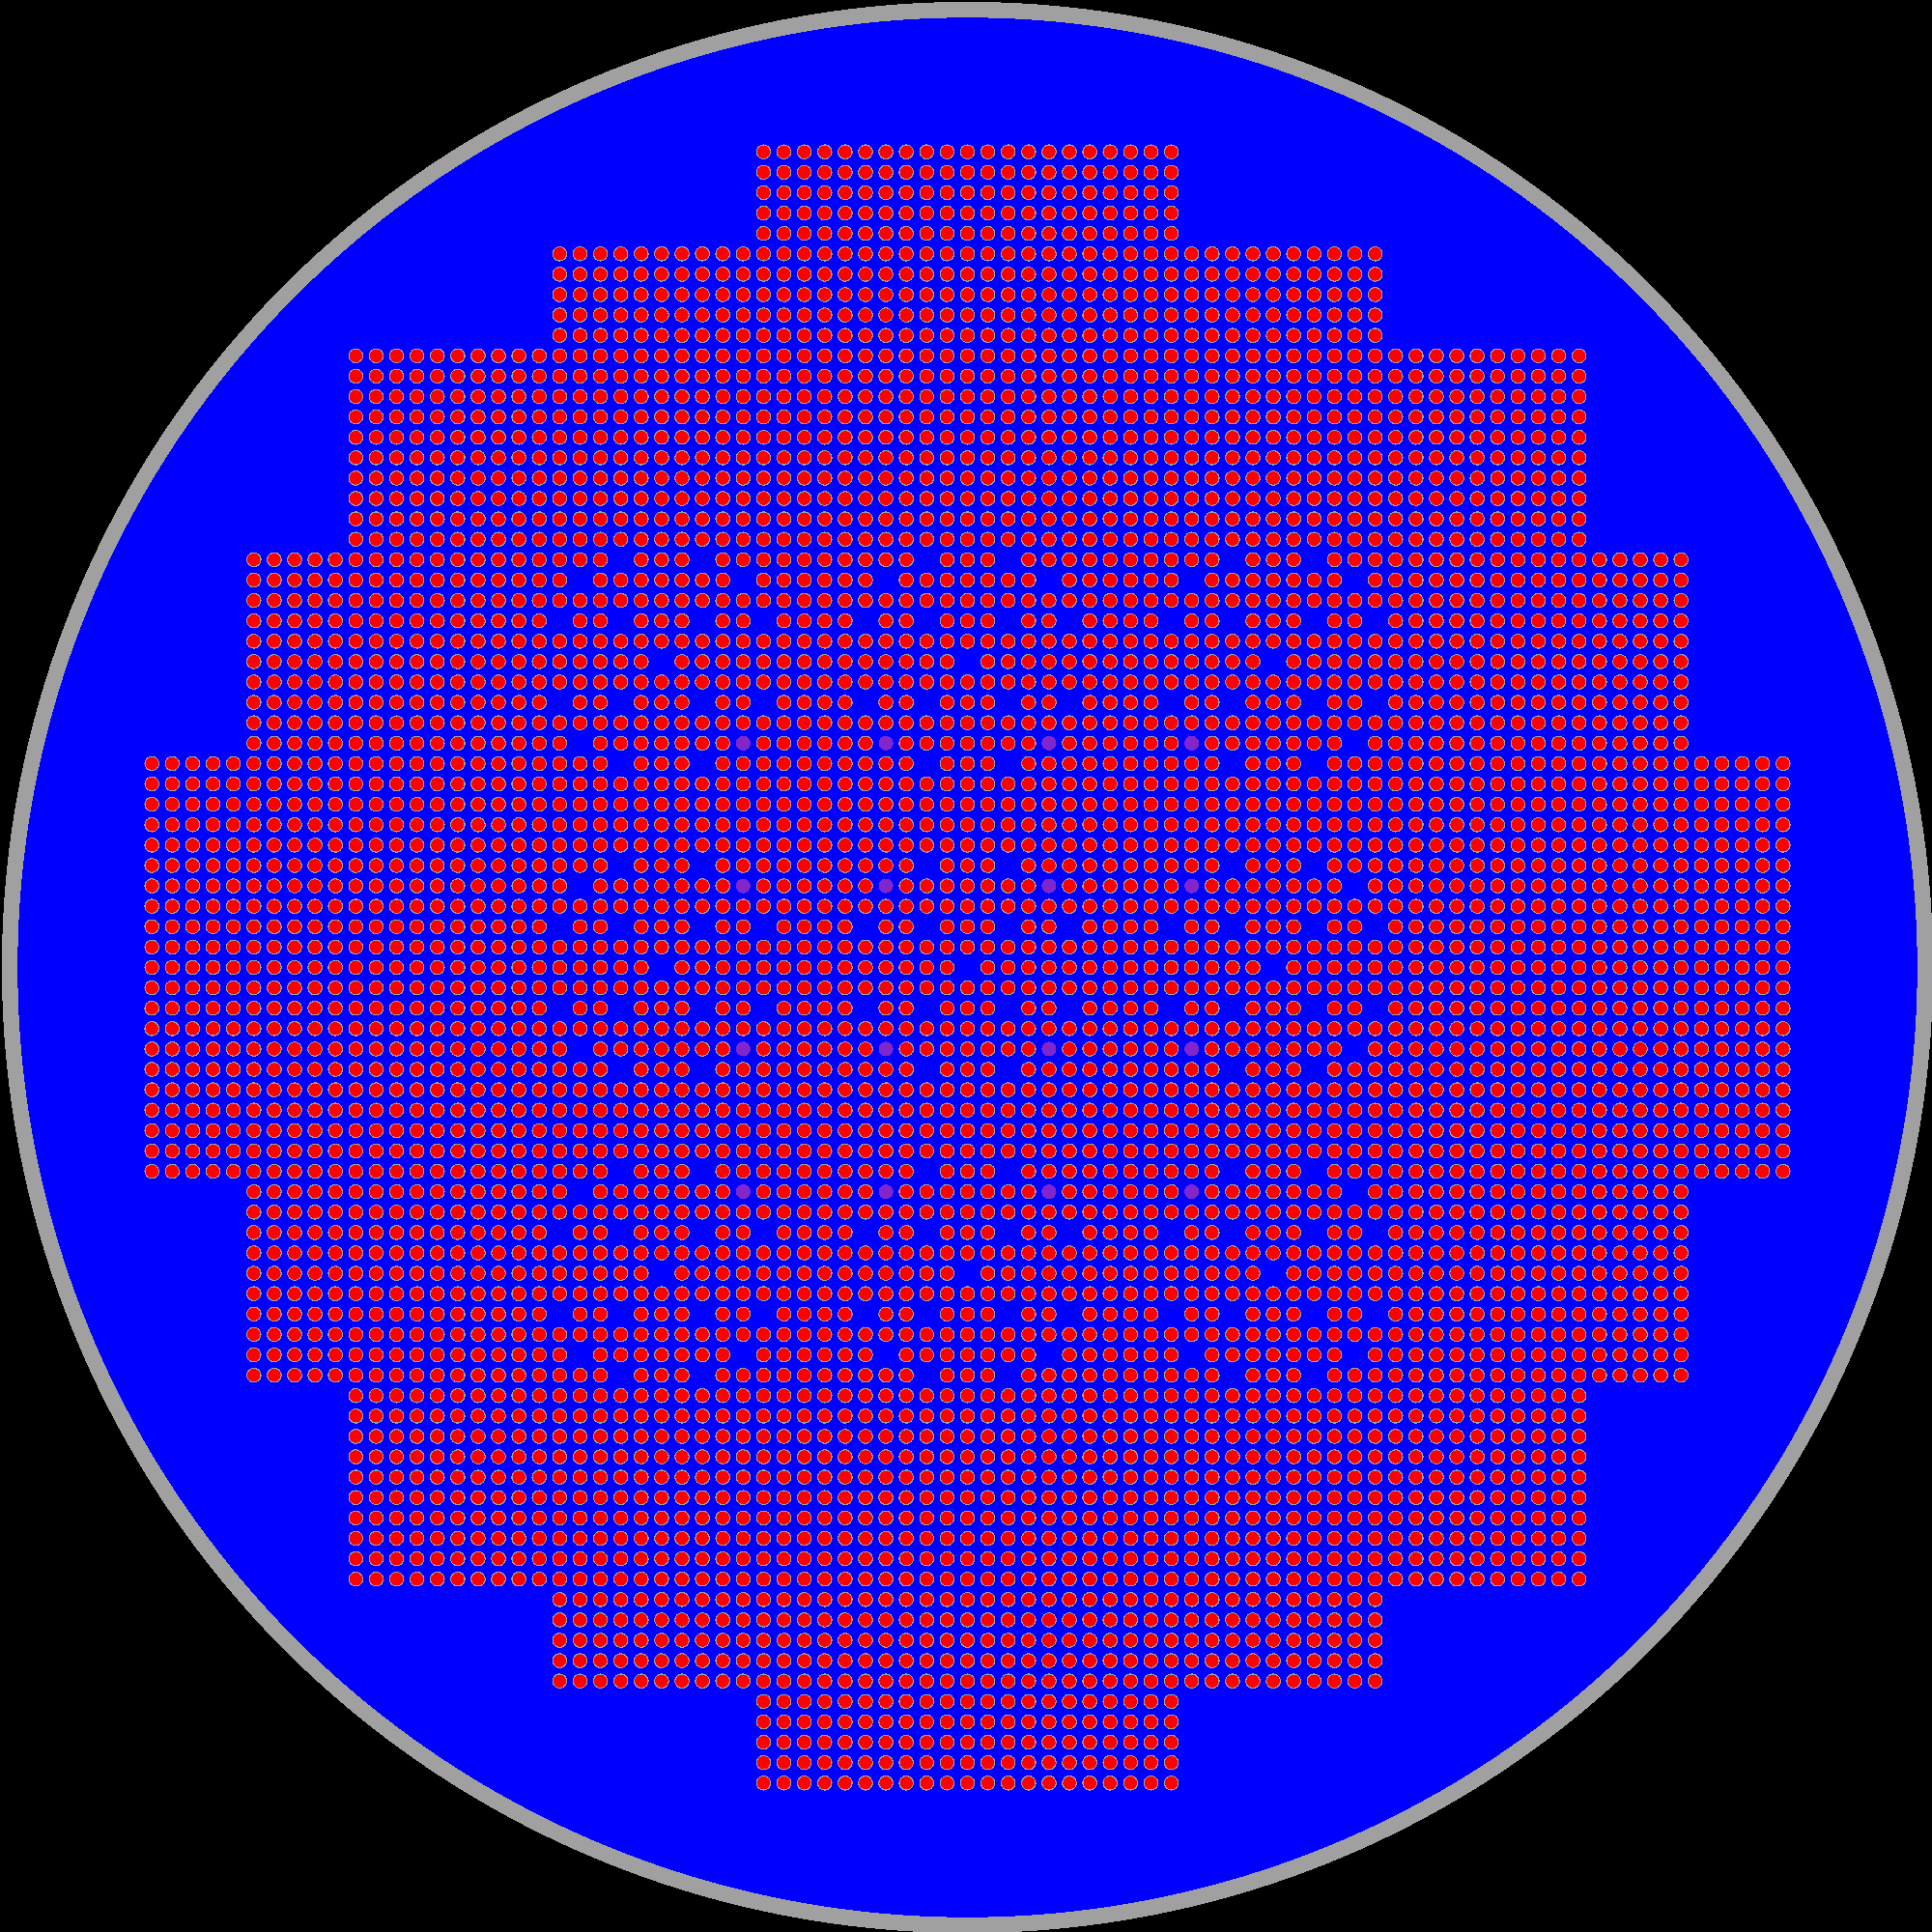
\includegraphics[width=2in]{src/plots/4_col_spec.png}
      \end{columns}
    \end{textblock}
  }
  
\end{frame}

%-------------------------------------------------------------------------------

\begin{frame}[fragile]{Plotting Options}

  \begin{scriptsize}
    \begin{lstlisting}[language=XML,gobble=4]
      <?xml version="1.0"?>
      <plots>
      
        <!-- Use a mask to plot only specific cells -->
        <plot id="5" type="slice" color="cell">
          <filename>col_spec</filename>
          <origin>0 0 0</origin>
          <width>155 155</width>
          <basis>xy</basis>
          <pixels>2000 2000</pixels>
          
          <!-- Here we plot only cells 31 and 1112, coloring all other cells white -->
          <mask components="31 1112" background="255 255 255"/>
          
          <!-- We can still set specific colors while using a mask -->
          <col_spec id="31" rgb="0 255 0"/>      <!-- Control: green  -->
          <col_spec id="1112" rgb="0 0 0"/>      <!-- Barrel:  black  -->
          
          <!-- we can still set the background color when using a mash -->
          <background>0 255 255</background>
        </plot>

      </plots>
    \end{lstlisting}
  \end{scriptsize}

  \begin{itemize}
    \item Use a mask to isolate features of interest
  \end{itemize}
  
  \onslide<2>{
    \setlength{\TPHorizModule}{\framewidth}
    \setlength{\TPVertModule}{\paperheight}
    \begin{textblock}{1}(0.12,-0.68)
      \begin{columns}[c]
      \column{2in}
      \column{3.5in}
      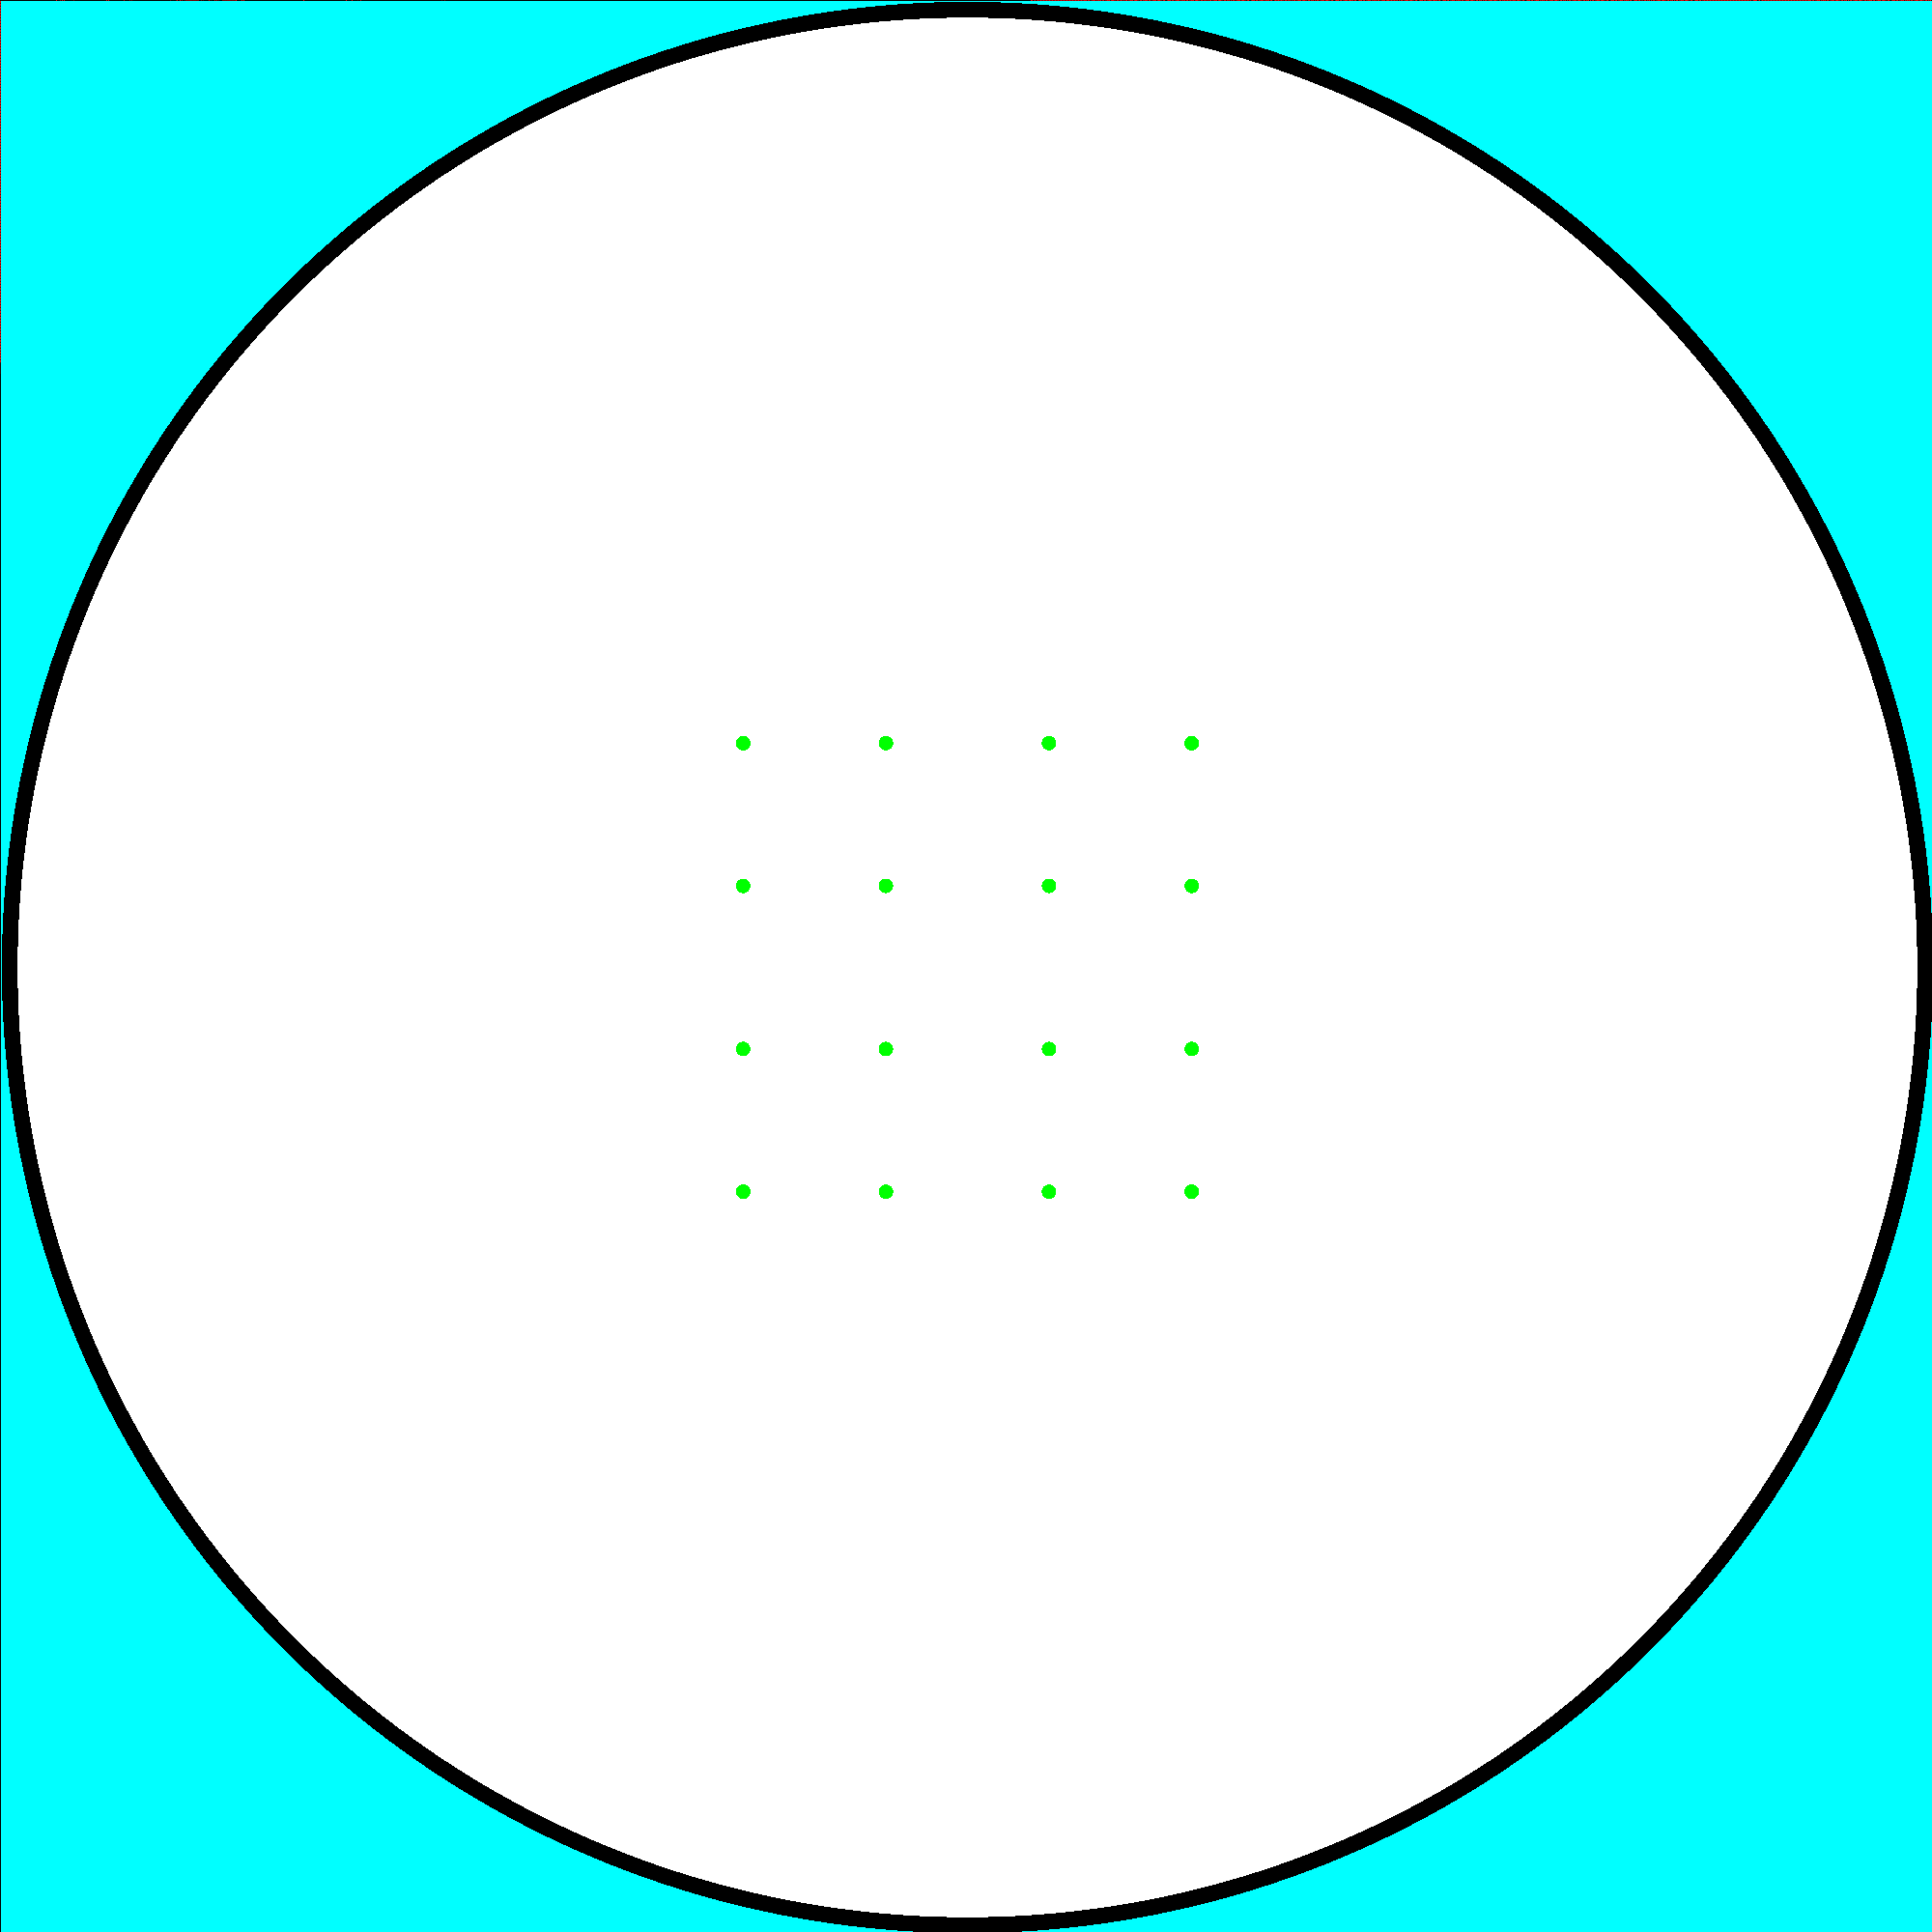
\includegraphics[width=2in]{src/plots/5_col_spec.png}
      \end{columns}
    \end{textblock}
  }
  
\end{frame}
